\section{Actions} \label{sec:action}
Actions are small graphical components associated with a \src{dockable}. They can show up at different locations, e.g. as buttons in the title.
\begin{figure}[ht]
\centering
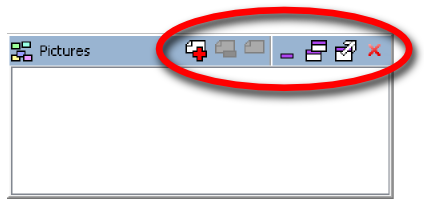
\includegraphics[scale=0.75]{actions/actions}
\caption{A set of actions on a \src{dockable}. The actions are the icons within the red oval.}
\label{fig:actions}
\end{figure}
An action is an instance of \src{CAction}. \src{Common} provides several subclasses of \src{CAction}. \src{CAction}s can be added to any \src{DefaultCDockable} through the method \src{addAction}. An example:
\begin{lstlisting}
DefaultCDockable dockable = ...
CAction action = new ...

dockable.addAction( action )
\end{lstlisting}

To separate a group actions from another group a separator is needed. The method \src{addSeparator} of \src{DefaultCDockable} adds such a separator. Separators are specialized \src{CAction}s.

An action is not a \src{Component}, it can appear at the same time at different locations with different views. For example an action can be seen as button in a title and at the same time as menu-item in a popup-menu.

\subsection{CButton}
\src{CButton}s are actions that can be triggered many times by the user and will always behave the same way. \src{CButton} itselfs is much like \src{JButton}s and offer many methods that can also be found in \src{JButton}s. E.g. clients can add an \src{ActionListener} to the \src{CButton} in order to be informed when the user clicks onto the button.

\subsection{CCheckBox}
This action has a state, it is either selected or not selected (\src{true} or \src{false}). Whenever the user triggers the action the state changes. \src{CCheckBox} is abstract and clients must create a subclass, the method \src{changed} will be called when the state changes. An example:
\begin{lstlisting}
public class SomeAction extends CCheckBox{
	public SomeAction(){
		setText( "Something" );
	}
	
	protected void action(){
		boolean selected = isSelected();
		...
	}
}
\end{lstlisting}

\subsection{CRadioButton}
In most aspects the \src{CRadioButton} behaves like a \src{CCheckBox}. \src{CRadioButton}s are grouped together, the user can select only one of the buttons in a group. A group is realized with the help of the class \src{CRadioGroup}:
\begin{lstlisting}
CRadioButton buttonA = ...
CRadioButton buttonB = ...

CRadioGroup group = new CRadioGroup();

group.add( buttonA );
group.add( buttonB );
\end{lstlisting}

\subsection{CMenu}
A \src{CMenu} is a list of \src{CAction}s. The user can open the \src{CMenu} and it will show a popup-menu with its actions. Clients can add and remove actions from a \src{CMenu} through methods like \src{add}, \src{insert}, or \src{remove}.

\begin{figure}[ht]
\centering
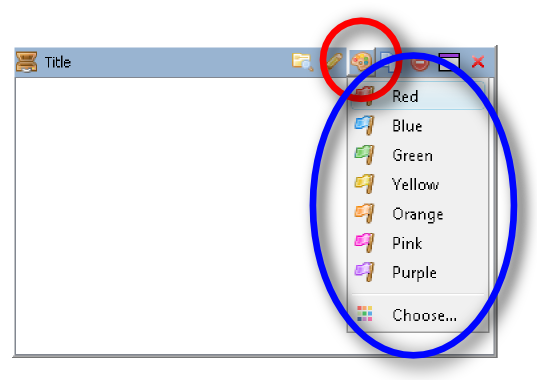
\includegraphics[scale=0.75]{actions/cmenu}
\caption{An open \src{CMenu}. The action itself is at the top within the red circle. Its menu consists of \src{CButton}s and a separator, the menu is within the blue oval.}
\label{fig:cmenu}
\end{figure}

\subsection{CDropDownButton}
A \src{CDropDownButton} consists of two buttons. One of them opens a menu, the other one triggers the last selected item of that menu again. 

\begin{figure}[ht]
\centering
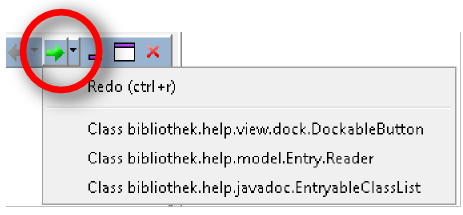
\includegraphics[scale=0.75]{actions/cdropdown}
\caption{A \src{CDropDownButton} within a red circle.}
\label{fig:cdropdown}
\end{figure}

The behavior of \src{CDropDownButton} can be influenced through its items. This requires that the items are subclasses of \src{CDropDownItem}. \src{CButton}, \src{CCheckBox} and \src{CRadioButton} fulfill this requirement. There are three properties to set:
\begin{itemize}
 \item \src{dropDownSelectable} - whether the action can be selected at all. If not, then clicking onto the item might trigger it, but the drop-down-buttons icon and text will remain unchanged.
 \item \src{dropDownTriggerableNotSelected} - if not set, then this item cannot be triggered if not selected. As a consequence the item must be clicked twice until it reacts.
 \item \src{dropDownTriggerableSelected} - if not set, then this item cannot be triggered if selected. It still can be triggered by opening the menu and then clicking onto the item.
\end{itemize}
If a \src{CDropDownButton} cannot trigger its selected item, then it just opens its menu.

\subsection{CPanelPopup}
Basically a button that opens a popup with an arbitrary component as content. The popup appears at the same location the menu of a \src{CMenu} would appear. In a menu a \src{CPanelPopup} appears as menu-item and opens the popup in the middle of the \src{CDockable} to which it is attached. The class provides methods for clients to modify its behavior, e.g. to replace the popup by another implementation.

\subsection{CBlank}
This action is not visible and does nothing. It can be used as placeholder where a \src{null} reference would cause problems, e.g. because \src{null} is sometimes replaced by some default value.

\subsection{System Actions}
\src{Common} adds a number of actions to any \src{CDockable}, e.g.: the close-button. These actions are deeply hidden within the system and cannot be accessed. There is however a mechanism to replace them with custom actions. Each \src{CDockable} has a method \src{getAction} which is called before a system action is put in place. If this method does return anything else than \src{null} then the system action gets replaced. \src{AbstractCDockable} offers the method \src{putAction} to set these replacements. An example:
\begin{lstlisting}
SingleCDockable dockable = ...
CAction replacement = ...

dockable.putAction( CDockable.ACTION_KEY_MAXIMIZE, replacement );
\end{lstlisting}
In this example whenever the maximize-action of \src{dockable} should be visible, \src{replacement} is shown. This feature should of course be treated with respect, changing the behavior of an action can confuse the user a lot.

\classbox{The class \src{CCloseAction} is an action that closes any \src{dockable} on which it is shown. The subclasses of \src{CExtendedModeAction} change the extended-mode of their \src{dockable}s.}

\subsection{Custom Actions}
Clients are free to write their custom actions. They need to implement a new \src{DockAction} and a subclass of \src{CAction}. The subclass can give its super-class an instance of the custom \src{DockAction} or call \src{init} to set the action. Please refere to the guide for \src{Core} to find out how to implement a \src{DockAction}.
 
